\chapter{\label{cap:metodologiaTecnicas}Metodología y técnicas}

Con la finalidad de realizar los experimentos pertinentes al proyecto de mi doctorado primero hay que preparar una nube de átomos fríos y generar las condiciones requeridas para tener un medio en condiciones de transparencia electromagnéticamente inducida. También es necesario montar los componentes necesarios para la detección de la imagen con la cual obtendremos información del cambio de fase. Posteriormente está el análisis de los datos que se comparará con simulaciones numéricas para obtener conclusiones.

\section{\label{sec:generacionRydberg}Generación de estados de Rydberg}

La producción de un medio con átomos en estado de Rydberg pasa, primero, por aislar a los átomos de interacciones externas y proporcionar un ambiente controlado. Durante el año 2021, en el laboratorio de Óptica Cuántica de Rydberg OCR (ver~\ref{sec:laboratorioOCR}), se hizo el armado y montaje del sistema de vacío cuya presión interna es menor a $\SI{10e-10}{\milli\bar}$~\cite{alonso}, dentro de la cámara de vacío se encuentran dispensadores que emiten gas de Rb al paso de una corriente en ellos. Esta cámara a ultra alto vacío suprime en gran medida las interacciones del gas de Rb con otras partículas a tal punto que se vuelven despreciables.

\subsection{\label{sub:mot}Trampa Magneto-Óptica}

\begin{wrapfigure}{r}{0.45\textwidth}
\vspace{-2\baselineskip}
\centering
\begin{minipage}{0.42\textwidth}
\centering
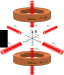
\includegraphics[width=0.65\linewidth]{MOT}  
\caption[Esquema de una MOT]{\label{fig:mot}Trampa Magneto-Óptica. Las bobinas producen un campo magnético cuadrupolar $\vektor{B}$ necesario para atrapar los átomos usando haces láser con la polarización adecuada, circular derecha $\sigma_\sm{+}$ o circular izquierda $\sigma_\sm{-}$.}
\end{minipage}
\end{wrapfigure}

Para enfriar a los átomos implementamos la técnica de \emph{Trampa Magneto-Óptica} (MOT, por sus siglas en inglés) que les valió el premio Nobel de Física a S. Chu, C. Tannougji y W. Phillips en 1997. Esta técnica ennfria una nube de átomos en tres dimensiones espaciales mediante tres pares de haces láser contrapropagantes y ortogonales entre sí. El confinamiento de estos átomos en una región del espacio, dada por la intersección de los seis haces, lo lleva a cabo la luz al interactuar con los átomos, cuya estructura interna está enriquecida por el desdoblamiento de sus niveles magnéticos debido a un campo cuadrupolar generado por un par de bobinas. Bajo estas circustancias podemos describir la interacción luz-materia como una fuerza viscosa que reduce la velocidad de los átomos, a la vez que restauradora que los mantiene atrapados, como si de un resorte se tratara.

\subsection{\label{sub:luzAnclaje}Luz láser y anclaje}

Otro aspecto importante es la estabilidad de los haces láser, tanto en potencia, modo espacial y frecuencia. En el laboratorio de OCR trabajamos con controladores para cada láser que mantiene una temperatura fija para los diodos láser y cuenta con la función de retroalimentación para fijar la frecuencia de los láseres. Entonces, como todo sistema de retroalimentación, es necesario contar con una referencia para su funcionamiento, en este caso una referencia en frecuencia. El sistema de láseres consta actualmente de 5 protagonistas, 4 láseres en el infrarrojo cercano y el quinto de luz azul:

\begin{itemize}
\item \textbf{Enfriamiento}: láser que utilizamos para crear los tres brazos ortogonales de luz de la MOT. Su frecuencia se ancla a la transición hiperfina $F=3\to F'=4$ del $\prescript{85}{}{\mathrm{Rb}}$ $\bigl(F=2\to F'=3\text{ para el }\prescript{87}{}{\mathrm{Rb}}\bigr)$, la cual denominamos \emph{transición de enfriamiento}. Posteriormente se desintoniza al rojo para enfriar los átomos~\cite{foot}.
\item \textbf{Rembombeo}: sintonizado en frecuencia con la transición $F=2\to F'=3$ del $\prescript{85}{}{\mathrm{Rb}}$ $\bigl(F=1\to F'=2\text{ para el }\prescript{87}{}{\mathrm{Rb}}\bigr)$, sirve para reingresar los átomos, cuya población haya pasado al nivel $F=2$ (o $F=1$), a la transición de enfriamiento.
\item \textbf{Imagen}: tiene las mismas características que el láser de enfriamiento salvo que este no se desintoniza, es resonante con la transición del rubidio para generar una imagen de absorción de la nube atómica.
\end{itemize}

\begin{wrapfigure}{l}{0.45\textwidth}
\vspace{-2\baselineskip}
\centering
\begin{minipage}{0.42\textwidth}
\centering
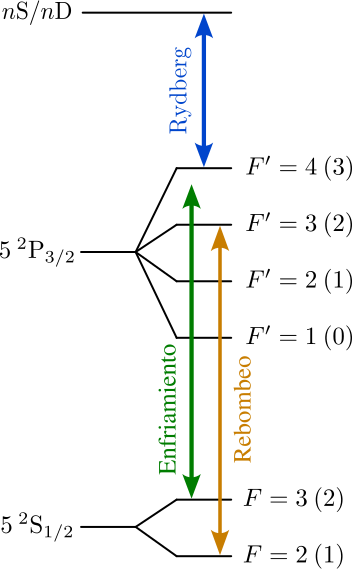
\includegraphics[width=0.65\linewidth]{transiciones}  
\caption[Transiciones del Rb]{\label{fig:transiciones}Transiciones involucradas en la MOT utilizando la línea $\mathrm{D}_\sm{2}$. Sin paréntesis los subniveles de $\prescript{85}{}{\mathrm{Rb}}$ y en paréntesis de $\prescript{87}{}{\mathrm{Rb}}$.}
\end{minipage}
\end{wrapfigure}

Los anteriores láseres se anclan tomando como referencia la frecuencia del que denominamos \textbf{láser maestro}: este láser está anclado en frecuencia a una cavidad mediante el método de Pound-Drever-Hall~\cite{black}, utilizando un modulador electro-óptico somos capaces de anclar el láser maestro a una frecuencia arbitraria y no sólo a las frecuencias del resonador cuya separación está fija por el \emph{rango espectral libre}~\cite{steck1}. El anclaje lo elegimos a la frecuencia del \emph{crossover} $3\otimes4$ del $\prescript{85}{}{\mathrm{Rb}}$ que corresponde a una longitud de onda de aproximadamente $\SI{780.244}{\nano\meter}$.

%en nuestro caso usamos un generador de funciones $f_\sm{\mathrm{GF}}$ y una DDS $f_\sm{\mathrm{DDS}}$ junto con un mezclador electrónico para mandar dos frecuencias a una de las dos entradas de un Modulador Electro-Óptico (EOM, por sus siglas en inglés) $f_\sm{\mathrm{GF}}+f_\sm{\mathrm{DDS}}$ y $\abs{f_\sm{\mathrm{GF}}-f_\sm{\mathrm{DDS}}}$. Si el láser maestro emite luz de la forma $E_\sm{0}=\E_\sm{0}e^{-j2\pi ft}$ que se envía a la otra entrada del EOM, este componente modula la fase del haz de la forma
%
%\begin{equation}
%\label{ec:modulacionFase}
%E=\E_\sm{0}\exp{\left\{-j2\pi\left[f+\beta_\sm{+}\sen{\left(f_\sm{\mathrm{GF}}+f_\sm{\mathrm{DDS}}\right)}+\beta_\sm{-}\sen{\abs{f_\sm{\mathrm{GF}}-f_\sm{\mathrm{DDS}}}}\right]t\right\}},
%\end{equation}
%
%para determinadas constantes $\beta_\sm{\pm}$ llamadas \emph{profundidad de modulación de fase}. Con ayuda de la identidad de Jacobi–Anger expandimos la expresión en la ecuación~\ref{ec:modulacionFase} para concluir que a la salida del EOM tenemos una onda cuyas componentes en frecuencia son: la frecuencia nominal del láser $f$, otras dos a una distancia $f_\sm{\mathrm{DDS}}$ de $f$ que llamamos bandas laterales, y otras cuatro frecuencias que son las bandas laterales de las bandas laterales anteriores y que distan $f_\sm{\mathrm{GF}}$ de estas últimas. Con estas bandas laterales y un resonador óptico podemos fijar la frecuencia del láser maestro a una frecuencia arbitraria y no sólo a las frecuencias del resonador cuya separación está fija por el \emph{rango espectral libre}~\cite{steck1}. El anclaje lo elegimos a la frecuencia del \emph{crossover} $3\otimes4$ del $\prescript{85}{}{\mathrm{Rb}}$ que corresponde a una longitud de onda de aproximadamente $\SI{780.244}{\nano\meter}$.

\p Finalmente tenemos el haz de luz azul que nombramos \textbf{láser de Rydberg}. Este se obtiene como resultado de enviar un haz de luz en el infrarrojo lejano a través de un cristal no lineal que dobla la frecuencia del campo incidente, reduciendo a la mitad la longitud de onda; dicho proceso es conocido como \emph{Generación del Segundo Armónico} (SHG, por sus siglas en inglés). El anclaje de este láser también se hace mediante la técnica de PDH y su controlador nos permite cambiar la frecuencia para elegir el nivel de Rydberg $n\mathrm{S}$ o $n\mathrm{D}$ que queramos excitar.

\section{\label{sec:controlEstadosAtomicos}Control de estados atómicos}

El ancho de línea de un nivel de energía es proporcional a la tasa de transición $\Gamma$, ésta a su vez es proporcional al cuadrado del elemento de matriz dipolar de esa transición según la regla de oro de Fermi. Así pues, de acuerdo con la tabla~\ref{tab:propiedadesRydberg}, el ancho de línea disminuye como $(n^{*})^{-3}$, al igual que el espaciamiento entre niveles de energía adyacentes. Lo anterior significa que los niveles de energía se juntan más y son más delgados entre mayor sea el nivel de Rydberg, por lo tanto, para lograr una situación predecible de los estados de Rydberg que excitamos en los experimentos es indispensable, por un lado, contar con láseres cuyo ancho de línea sea más delgado que el ancho de línea de las transiciones atómicas. Usamos una cavidad de \emph{ultrabaja expansión} (ULE, por sus siglas en inglés) y alta fineza para anclar el láser de Rydberg, de esta forma el ancho de línea de la luz azul para excitar a estados de Rydberg es sumamente delgado ya que se ancla al máximo del pico de transmisión de la cavidad, cuyo ancho completo a media altura (FWHM, por sus siglas en inglés) es del orden de cientos de $\si{\kilo\hertz}$. Según nuestras mediciones~\cite{eduardo}, la fineza y el FWHM de nuestra cavidad ULE para $\SI{960}{\nano\meter}$ es $\mathcal{F}=\SI{13617\pm7}{}$ y $\nu_\sm{\mathrm{FWHM}}=\SI{109.91\pm0.06}{\kilo\hertz}$.

% Anclar el láser al máximo del pico lo hace más delgado que el ancho del pico de transmisión. No podemos medir el ancho de línea del haz de Rydberg, para ello creo recordar que necesitamos una fibra de varios kilómetros de longitud.

\p Por otro lado, necesitamos controlar de mejor manera la población en los estados atómicos, en concreto en los subniveles magnéticos $m_\sm{F}$, pues hay muchos niveles involucrados y esto resulta en una dinámica muy compleja, sumado a que después del enfriamiento y confinamiento con la MOT los átomos no se encuentran, en conjunto, en un estado bien definido. El láser de rebombeo en un ejemplo del control de la población, en este caso, para enfriar eficazmente a los átomos. Sin embargo, la población se distribuye en las diferentes proyecciones $m_\sm{F}$ de la estructura hiperfina de los átomos, en otras palabras, hay varias vías de excitación posible con dos fotones para ir desde el estado base a un estado de Rydberg puesto que tenemos una mezcla estadística de las proyecciones mágnéticas $m_\sm{F}$, en la figura~\ref{fig:transiciones87Rb} ilustramos todos los caminos para una excitación de Rydberg del $\prescript{87}{}{\mathrm{Rb}}$. Es necesario implementar un bombeo óptico para definir muy bien el subnivel magnético de los átomos en nuestros experimentos.

\begin{figure}[H]
\centering
\begin{minipage}{0.8\textwidth}
\centering
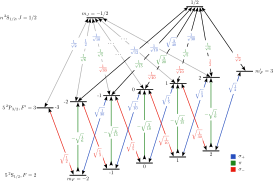
\includegraphics[width=0.8\textwidth]{transiciones87Rb}
\caption{\label{fig:transiciones87Rb}Modelo de átomo de tres niveles en escalera del $\prescript{87}{}{\mathrm{Rb}}$. Se muestran los subniveles magnéticos de la estructura hiperfina para el estado base y el primer estado excitado, para el estado de Rydberg basta considerar la estructura fina.}
\end{minipage}
\end{figure}

\subsection{\label{sub:bombeoOptico}Bombeo Óptico}
 
Utilizaremos \emph{bombeo óptico} para mantener a todos los átomos en un estado de momento magnético bien definido. En presencia de un campo magnético se desdoblan los niveles hiperfinos de los átomos de Rb, es decir, se rompe la degeneración dando lugar a los subniveles magnéticos o niveles Zeeman. Al mandar luz con una frecuencia y polarización definida se van \emph{bombeando} estos subniveles, por ejemplo, con un haz láser para la transición del estado base al primer estado excitado con polarización $\sigma_\sm{+}$, el electrón es bombeado al nivel $m_\sm{F}=2$. La razón está en que la emisión espontánea y estimulada obedece $\Delta m_\sm{F}=0,\pm1$, en el proceso de bombeo el electrón estará en el nivel $m_\sm{F}=2$, cuya transición con el haz polarizado es hacia $m_\sm{F'}=3$ del primer estado excitado, y de este estado sólo puede pasar nuevamente a $m_\sm{F}=2$.

\p Dicho lo anterior, es importante el valor y orientación del campo magnético externo que desplaza los niveles Zeeman, por ello es necesario la construcción de unas bobinas que nos den un valor de campo constante (configuración de Helmholtz) y que al mismo tiempo compensen el campo magnético terrestre.

\section{\label{sec:densidadOptica}Densidad Óptica}

La \emph{Densidad Óptica} $\OD$ de un medio mide su capacidad de reducir la potencia de la luz que lo atraviesa, está relacionada con la transmitancia del medio $T$ por $\OD=-\ln(T)$. Varias medidas experimentales depende del valor de la $\OD$ del medio, en nuestro caso es relevante poder manipular su valor, puesto que la velocidad de grupo y el retraso que experimenta un pulso láser es inversa y directamente proporcional a la densidad óptica del medio, respectivamente.

\p El bombeo óptico que presentamos anteriormente nos ayuda a aumentar la $\OD$ de la nube de átomos, puesto que su probabilidad de excitación es mayor comparado a una nube atómica con una mezcla estadística de los niveles Zeeman.

\subsection{\label{sub:trampaDipolar}Trampa Dipolar}

Sumado al bombeo óptico, una \emph{Trampa Dipolar} servirá para tener control en la $\OD$ de la nube. El principio de funcionamiento de estas trampas está en la interacción dispersiva de la luz con el momento dipolar que ésta induce en los átomos~\cite{grimm}. La fuerza derivada de dicha interacción es conservativa, en contraste con la MOT cuya fuerza es disipativa ya que se usa para enfriar. Entonces, se utiliza el máximo del potencial para atrapar a los átomos, en este caso, el máximo de intensidad del láser $I(\vektor{r})$:

\begin{equation}
\label{ec:fuerzaDipolar}
F_\sm{\mathrm{dip}}(\vektor{r})=\dfrac{1}{2\epsilon_\sm{0}c}\Re{\left(\alpha_\sm{E}\right)}\nabla I(\vektor{r}).
\end{equation}

Con este tipo de fuerza, dependiente del perfil de intensidad del láser, podemos configurar trampas que atrapen a los átomos según el perfil, incluyendo arreglos casi unidimensionales o alargados en una dirección, lo cual aumentará no sólo la densidad atómica sino también la densidad óptica del medio. A su vez, como vimos en~\ref{sub:luzLenta}, el ensanchamiento de la nube en la dirección en la que se propagarán los pulsos de luz incrementará su retraso a la detección.

\section{\label{sec:medicionesFase}Mediciones de fase}

Una forma de cuantificar la interacción entre la luz y la materia es midiendo los cambios que sufre la luz al atravesar el medio atómico, estos cambios se manifiestan en modificaciones de las amplitudes y las fases de las ondas que componen el haz de luz. Monitorear la amplitud se hace de forma directa con la detección de la luz que pasa por los átomos, la corriente registrada en el detector es proporcional a la intensidad de la luz, que a su vez es proporcional al cuadrado de la amplitud; normalizando lo anterior con una medición similar pero sin átomos, es decir, con la amplitud del haz sin modificarse por el medio atómico, obtenemos la \emph{transmitancia} del ensamble de átomos. La transmitancia depende del medio por el cual pasa la luz y existen algunas derivaciones teóricas para modelarlal, como la \textbf{ley de Beer-Lamber}~\cite{bornWolf}, válida para ensambles cuya absorción sea proporcional a su densidad y a la distancia que recorre la luz dentro de estos.

\p Para fines de mi proyecto, lo más interesante está en el cambio en la fase, puesto que queremos medir como responde un haz láser atravesando el conjunto de átomos en condiciones de EIT. Como vimos en~\ref{sub:eit}, el ensamble de átomos se vuelve transparente, por que que la amplitud del campo de la luz no se altera. Lo que es más, la luz atraviesa el medio que es muy dispersivo (gradiente respecto a la frecuencia del índice de refracción). Dado que los detectores solamente pueden medir intensidades, es necesario utilizar técnicas para mapear el cambio de fase a la amplitud del campo y así extraer la información requerida.

\subsection{\label{sub:deteccionHomodina}Detección homodina}

Una técnica para obtener el cambio de fase de una onda es la nombrada \emph{detección homodina}, que consiste en medir la información de fase de un haz láser al compararlo con otro haz de referencia de la misma frecuencia, de ahí su nombre. Se denomina \textbf{señal} al campo de luz cuya fase queremos conocer $E_\sm{\mathrm{S}}(t)$, mientras que el campo de referencia y cuya fase es conocida o se puede controlar muy bien se llama \textbf{oscilador local} $E_\sm{\mathrm{OL}}(t)$.

\begin{figure}[H]
\centering
\begin{minipage}{0.8\textwidth}
\centering
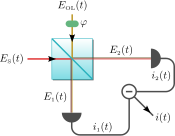
\includegraphics[width=0.4\textwidth]{deteccionHomodina}
\caption{\label{fig:deteccionHomodina}Vista esquemática de la detección homodina. Antes de la detección se controla la fase $\varphi$ del oscilador local y la información de la señal se recupera a partir de la diferencia de las fotocorrientes.}
\end{minipage}
\end{figure}

Ambos haces de entrada se hacen pasar por un \emph{divisor de haz}, los haces de salida $E_\sm{1}(t)$ y $E_\sm{2}(t)$, que son detectados y generan las fotocorrientes $i_\sm{1}(t)$ y $i_\sm{2}(t)$ respectivamente, son el resultado de la superposición de la transmisión de uno de los campos entrantes y la reflexión del otro campo (fig.~\ref{fig:deteccionHomodina}). La relación entre la salida y la entrada se puede expresar con la siguiente ecuación matricial~\cite{saleh}:

\begin{equation}
\label{ec:divisorHaz}
\begin{pmatrix}
E_\sm{1}(t)\\
E_\sm{2}(t)
\end{pmatrix}
=
\begin{pmatrix}
\T & \R'\\
\R & \T' 
\end{pmatrix}
\begin{pmatrix}
E_\sm{\mathrm{OL}}(t)\\
E_\sm{\mathrm{S}}(t)
\end{pmatrix},
\end{equation}

con $\T, \T', \R, \R'$ los coeficientes de transmisión y reflexión del divisor de haz. En general, estos coeficientes son cantidades complejas y son distintos para cada uno de los haces de luz de entrada. Si supones un material que ideal sin pérdidas para el divisor de haz, entonces la intensidad total a la entrada y la intensidad total a la salida es igual, esto es

\begin{equation}
\label{ec:conservacionEnergia}
\abs{E_\sm{\mathrm{OL}}(t)}^{2}+\abs{E_\sm{\mathrm{S}}(t)}^{2}=\abs{E_\sm{1}(t)}^{2}+\abs{E_\sm{2}(t)}^{2}.
\end{equation}

La anterior ecuación de conservación de energía se puede utilizar para probar las siguientes expresiones

\begin{equation}
\label{ec:igualdadModulos}
\abs{\T'}=\abs{\T},\quad\abs{\R'}=\abs{\R},\quad\abs{\T}^{2}+\abs{\R}^{2}=1,
\end{equation}

\begin{equation}
\label{ec:relacionFase}
\T'\R^{*}+\T^{*}\R'=0.
\end{equation}

Las ecuaciones en~\ref{ec:igualdadModulos} relacionan las magnitudes de los elementos de la matriz en~\ref{ec:divisorHaz} para un material sin pérdidas, mientras que~\ref{ec:relacionFase} relaciona sus argumentos. Si ahora también suponemos que el divisor de haz es simétrico, directamente los coeficientes de transmisión y reflexión son iguales y no sólo los módulos como apunta la expresión en~\ref{ec:igualdadModulos}. Con lo anterior obtenemos, a partir de la ecuación~\ref{ec:relacionFase}, que para un divisor de haz simétrico sin pérdidas las fases entre los coeficientes de transmisión $\T=\abs{T}e^{j\phi_{T}}$ y reflexión $\R=\abs{R}e^{j\phi_{R}}$ cumplen que

\begin{equation}
\label{ec:restriccionFase}
\cos{\left(\phi_\sm{T}-\phi_\sm{R}\right)}=0,
\end{equation}

por lo que la fase relativa entre la onda transmitida y la onda reflejada por un divisor de un haz de entrada es de $\pi/2$. Por conveniencia se elige $\phi_\sm{T}=0$, de ahí que la onda reflejada adquiera un cambio de fase $\pi/2$ para garantizar la unitariedad de la matriz de transformación en~\ref{ec:divisorHaz}. Si el divisor de haz es balanceado, es decir, que transmite el $50\%$ de la luz y refleja el otro $50\%$, lo que denominamos divisor de haz $50/50$, entonces $\T=1/\sqrt{2}$, $\R=j/\sqrt{2}$ y utilizando la ecuación~\ref{ec:divisorHaz} tenemos que la diferencia en las fotocorrientes $I(t)\propto\abs{E_\sm{1}(t)}^{2}-\abs{E_\sm{2}(t)}^{2}$ es

\begin{equation}
\label{ec:fotocorriente}
i(t)\propto2\Im{\left[E_\sm{\mathrm{OL}}^{*}(t)E_\sm{\mathrm{S}}(t)\right]}.
\end{equation}

Sean $E_\sm{\mathrm{OL}}(t)=\E_\sm{\mathrm{OL}}e^{j\varphi}e^{j\left(\omega t+\phi_{0}\right)}$ y $E_\sm{\mathrm{S}}(t)=\E_\sm{\mathrm{S}}e^{j\left(\omega t+\phi\right)}$  los campos de entrada de la misma frecuencia, con $\varphi$ la fase que introducimos al oscilador local y que controlamos, entonces la corriente $i(t)$ es
	
\begin{equation}
\label{ec:fotocorrienteFase}
i(t)\propto2\E_\sm{\mathrm{OL}}\E_\sm{\mathrm{S}}\sen{\left(\phi-\phi_\sm{0}-\varphi\right)},
\end{equation}

por ende, al conocer la fase del oscilador local y variar la fase $\varphi$ es posible conocer la fase de la señal con un ajuste a la función de fotocorriente $i(t)$ detectada.

\subsection{\label{sub:contrasteFase}Contraste de fase}

Otro método para conocer el cambio de fase que sufre una onda al cruzar un medio transparente es la \emph{imagen por contraste de fase}, que es uno de varios métodos dispersivos para medir fases. En esta sección abordaremos este método y veremos que puede ser visto como un  caso particular de detección homodina. Supongamos un medio transparente en $z=0$, una onda plana que se propaga en la dirección $z$ y cuya expresión justo antes del medio $z\to0^{-}$ es $E_\sm{i}(z\to0^{-},t)=\E_\sm{0}\cos{\left(\omega t\right)}$, el medio induce en la onda una fase dependiente de la posición $\phi(x,y)$, resultando en una onda de fase modulada:

\begin{equation}
\label{ec:ondaFaseModulada}
\begin{split}
\left.E_\sm{\mathrm{FM}}\left(\vektor{r},t\right)\right|_\sm{z=0}= & \hspace{1.5mm}\E_ \sm{0}\cos{\left[\omega t+\phi(x,y)\right]}\\
& \hspace{1.5mm}\E_\sm{0}\cos{\left(\omega t\right)}\cos{\left[\phi(x,y)\right]}+\E_\sm{0}\sen{\left(\omega tx\right)}\sen{\left[\phi(x,y)\right]}.
\end{split}
\end{equation}

Observamos que la expresión en~\ref{ec:ondaFaseModulada} es una onda de amplitud constante, suponiendo que las aberraciones del sistema de imagen (lentes y otros elementos ópticos) es despreciable, entonces el campo en el plano conjugado de imagen es esencialmente el mismo que en~\ref{ec:ondaFaseModulada}. Además, para valores pequeños de $\phi(x,y)$ y utilizando la segunda forma en la ecuación~\ref{ec:ondaFaseModulada} tenemos

\begin{equation}
\label{ec:ondaFasePequena}
E_\sm{\mathrm{FM}}\left(x,y,t\right)=\E_\sm{0}\cos{\left(\omega t\right)}+\E_\sm{0}\phi(x,y)\sen{\left(\omega t\right)},	
\end{equation}

el segundo término en la ecuación de arriba depende del medio pero el primer término no lo hace, es decir, es la parte no dispersada por el medio. Si logramos cambiar la fase relativa entre estos términos exactamente por $\pi/2$, cambiando el coseno a seno (o viceversa):

\begin{equation}
\label{ec:ondaFaseAmplitud}
E_\sm{\mathrm{FM}}\left(x,y,t\right)=\E_\sm{0}\left[1+\phi(x,y)\right]\sen{\left(\omega t\right)},	
\end{equation}

la cual es una onda de amplitud modulada cuya intensidad es proporcional a $1+2\phi(x,y)$, ergo podemos conocer el cambio de fase debido a un medio transparente midiendo la amplitud de la onda que resulta de cambiar por $\pi/2$ la fase, en este caso, de la porción de onda que no se dispersa. Para conseguir lo anterior se utiliza una \emph{lámina de fase}, una placa de un material transparente e índice de refracción $n_\sm{g}$, ésta se coloca en el plano de Fourier~\cite{hecht} del sistema de imagen para cambiar la fase de la luz no dispersada, dependiendo de la composición particular del sistema de imagen será la forma de la lámina de fase. Para una onda plana y una única lente, la porción que no es dispersada se enfoca en el plano de Fourier, una lámina de fase en cuyo centro haya una hendidura de una distancia $d$ tal que el $\left(n_\sm{g}-1\right)d=\lambda_\sm{0}/4$ basta para lograr el cambio de fase deseado. Otra forma es una onda plana que atraviesa un diafragma anular a la entrada del sistema de imagen, en el plano de Fourier la parte no dispersada forma igualmente un anillo, siendo está la forma que ha de tener una lámina de fase en tal sistema~\cite{hecht}.

\p Este método de imagen puede considerarse una detección homodina en cierto sentido, en la cual la luz no dispersada es el oscilador local y la señal el campo de radiación dispersado, donde se introduce una fase $\pi/2$ al oscilador local. Las diferencias que existen entre ambos métodos es que en la imagen por contraste de fase no hay un divisor de haz y se utiliza un solo detector.

\section{\label{sec:luzLentaDeteccionNoDestructiva}Luz lenta y detección no destructiva}

Aprovecharemos que la luz es \emph{lenta} dentro del medio atómico (ver~\ref{sub:luzLenta}) para medir el retraso de pulsos láser y caracterizar dicho medio, puesto que este retraso depende de la profundidad de la nube atómica y la velocidad de propagación en el medio. Utilizaremos un fotodiodo para detectar los pulsos de luz, primero sin átomos atrapados ($v_\sm{g}=c$) y luego con la nube altamente dispersiva en condiciones de EIT. Dado que el espectro de frecuencias de un pulso de luz con perfil temporal cuadrado es muy grande, pues son necesarias demasiadas frecuencias para reconstruirlo, la dispersión del medio afecta de forma distinta el retraso del pulso dependiendo de su componente en frecuencia, como resultado es muy complicado dar un valor preciso al retraso del pulso. Por lo anterior, los pulsos de luz se mandarán con un perfil temporal gaussiano para reducir el número de frecuencias requeridas para reconstuirlos.

\p Para efectuar mediciones verdaderamente no destructivas de la nube de átomos y caracterizarla, mandaremos dos pulsos láser, uno en resonancia dentro de la ventana de transparencia (fig.~\ref{fig:eitDispersion}), que será el pulso de luz lenta, y otro muy fuera de resonancia para que no sea absorbido ni dispersado por los átomos. Para un pulso con una velocidad de grupo de $v_\sm{g}=\SI[per-mode=symbol]{1000}{\meter\per\second}$ y una nube de $L=\SI{500}{\micro\meter}$ de profundidad, el retraso es alrededor de $\Delta t=\SI{500}{\nano\second}$ (ec.~\ref{ec:retraso}), por lo tanto un fotodiodo con un ancho de banda de $\SI{150}{\mega\hertz}$, como los que tenemos en el laboratorio, puede resolver estas diferencias temporales.